\documentclass[sigconf,anonymous,review]{acmart}

% WWW 2027 Research Full Paper review template.
% Keep the official ACM margins/fonts unchanged.
% Main paper: 8 pages. References + optional appendix allowed up to 12 pages total.

\AtBeginDocument{%
  \providecommand\BibTeX{{Bib\TeX}}}

% Avoid camera-ready copyright/reference metadata during anonymous review.
\setcopyright{none}
\settopmatter{printacmref=false}
\renewcommand\footnotetextcopyrightpermission[1]{}

\ifdefined\ifevalshowpending\else
  \expandafter\newif\csname ifevalshowpending\endcsname
  \evalshowpendingtrue
\fi
\providecommand{\evalpending}[2]{%
  \ifevalshowpending
    \par\smallskip\noindent
    {\small\textit{Pending---#1:} #2\par}\smallskip
  \fi
}
% Helpful packages. Add more only when needed.
\usepackage{booktabs}
\usepackage{amsmath}
\usepackage{microtype}
\usepackage{xspace}
\usepackage{algorithm}
\usepackage{algpseudocode}
\setcopyright{none}

\acmConference[The Web Conference 2027]
  {The ACM Web Conference 2027}
  {May 10--14, 2027}
  {Dublin, Ireland}

\begin{document}

\title{SPARE: Selective Prefill Scheduling to Improve Throughput and Latency in LLM Serving}

% Double-blind review: do not add real names, affiliations, acknowledgments,
% identifying repository URLs, or identifying self-citations here.
\author{Anonymous Author(s)}

\begin{abstract}
As AI search and agentic services become increasingly prevalent, these interactive Web applications require large language model (LLM) serving systems to deliver high throughput and low latency under GPU memory constraints. However, prefill-first schedulers may incur costly KV-cache evictions and recomputation by aggressively admitting new requests, while decode-first schedulers may delay new prefills and increase request latency. These competing priorities make it challenging to maximize serving throughput while meeting constraints on mean initial response latency, measured by time to first token (TTFT). We observe that aggressively prioritizing either prefill or decode is not always beneficial; instead, selectively deferring prefills can reduce execution interference and improve serving capacity. Motivated by this insight, we propose SPARE, a KV-cache-aware online scheduler that combines selective prefill deferral with progress-aware protection to mitigate costly evictions. Evaluations across diverse workloads and KV-cache configurations demonstrate that SPARE achieves up to 2.65$\times$ the serving capacity of baseline schedulers under the same mean TTFT constraint. Furthermore, in separate comparisons at matched request arrival rates, SPARE reduces mean TTFT by up to 82.1\%. Our code is publicly available at \url{https://anonymous.4open.science/r/SPARE-8963}
\end{abstract}

% ACM CCS Concepts
% Replace these examples with generated ACM CCS codes.
\begin{CCSXML}
<ccs2012>
   <concept>
       <concept_id>10010520.10010521.10010537.10003100</concept_id>
       <concept_desc>Computer systems organization~Cloud computing</concept_desc>
       <concept_significance>500</concept_significance>
       </concept>
 </ccs2012>
\end{CCSXML}

\ccsdesc[500]{Computer systems organization~Cloud computing}

% Keywords
\keywords{Large Language Model Serving, KV-Cache-Aware Scheduling, Prefill Deferral}

\maketitle

\section{Introduction}
\label{sec:introduction}


Large language models (LLMs)~\cite{openai2023gpt4,touvron2023llama2} increasingly power interactive Web applications such as AI search and agentic services, where serving systems must sustain high request throughput while delivering timely responses. High throughput keeps serving costs manageable, whereas low latency is essential to interactive user experience. Batching improves GPU utilization, but heterogeneous requests with different input and output lengths compete for computation and finite key-value (KV) cache space, creating interference between these objectives \cite{intro_vllm,intro_sarathi}. Such contention makes the timing of scheduling decisions consequential. 
A broader body of research in operations research and economics
likewise examines the value of strategically delaying decisions
when immediate actions constrain future opportunities
\cite{intro_baron2014,intro_akbarpour2020,intro_kerimov2024}.
 In LLM serving, sustaining high serving capacity while meeting latency objectives under limited GPU memory has therefore become a key scheduling problem.

The difficulty lies in the timing of prefill and decode work. Prefill processes a request's input before its first output token, after which decode generates subsequent tokens. Chunked prefill divides long inputs across iterations so that prefill and decode work can share a batch \cite{intro_sarathi}. Prefill and decode compete for shared computation and KV-cache resources, yet contribute differently to service latency: advancing prefill brings waiting requests closer to their first responses, whereas advancing decode sustains token generation for requests already being served. Aggressively advancing prefills can therefore interfere with ongoing decoding in several ways. First, additional prefill work lengthens an iteration and can stall ongoing generation \cite{intro_sarathi}. Second, a prefill that remains unfinished after an iteration retains its newly allocated KV blocks without yet producing a first token. Third, as multiple unfinished prefills expand concurrently, KV pressure can force later requests to wait or running requests to be preempted and subsequently recomputed. Conversely, excessive prefill deferral increases first-token waiting, even when it protects ongoing decoding. Under sustained load, these effects compound: requests accumulate, latency increases, and the arrival rate that the system can stably sustain decreases. The operational importance of sufficient serving capacity is visible in production systems. On July 30, 2026, OpenAI reported that some users could not start or continue ChatGPT conversations because the available processing capacity was insufficient for the required work \cite{intro_openai2026capacity}. Accordingly, we consider both \emph{latency}, measured primarily by mean time to first token (TTFT) at matched arrival rates, and \emph{serving capacity}, defined as the highest arrival rate that satisfies mean-TTFT, P99 time-between-token (TBT), and backlog-stability requirements.

\begin{figure}[t]
\centering
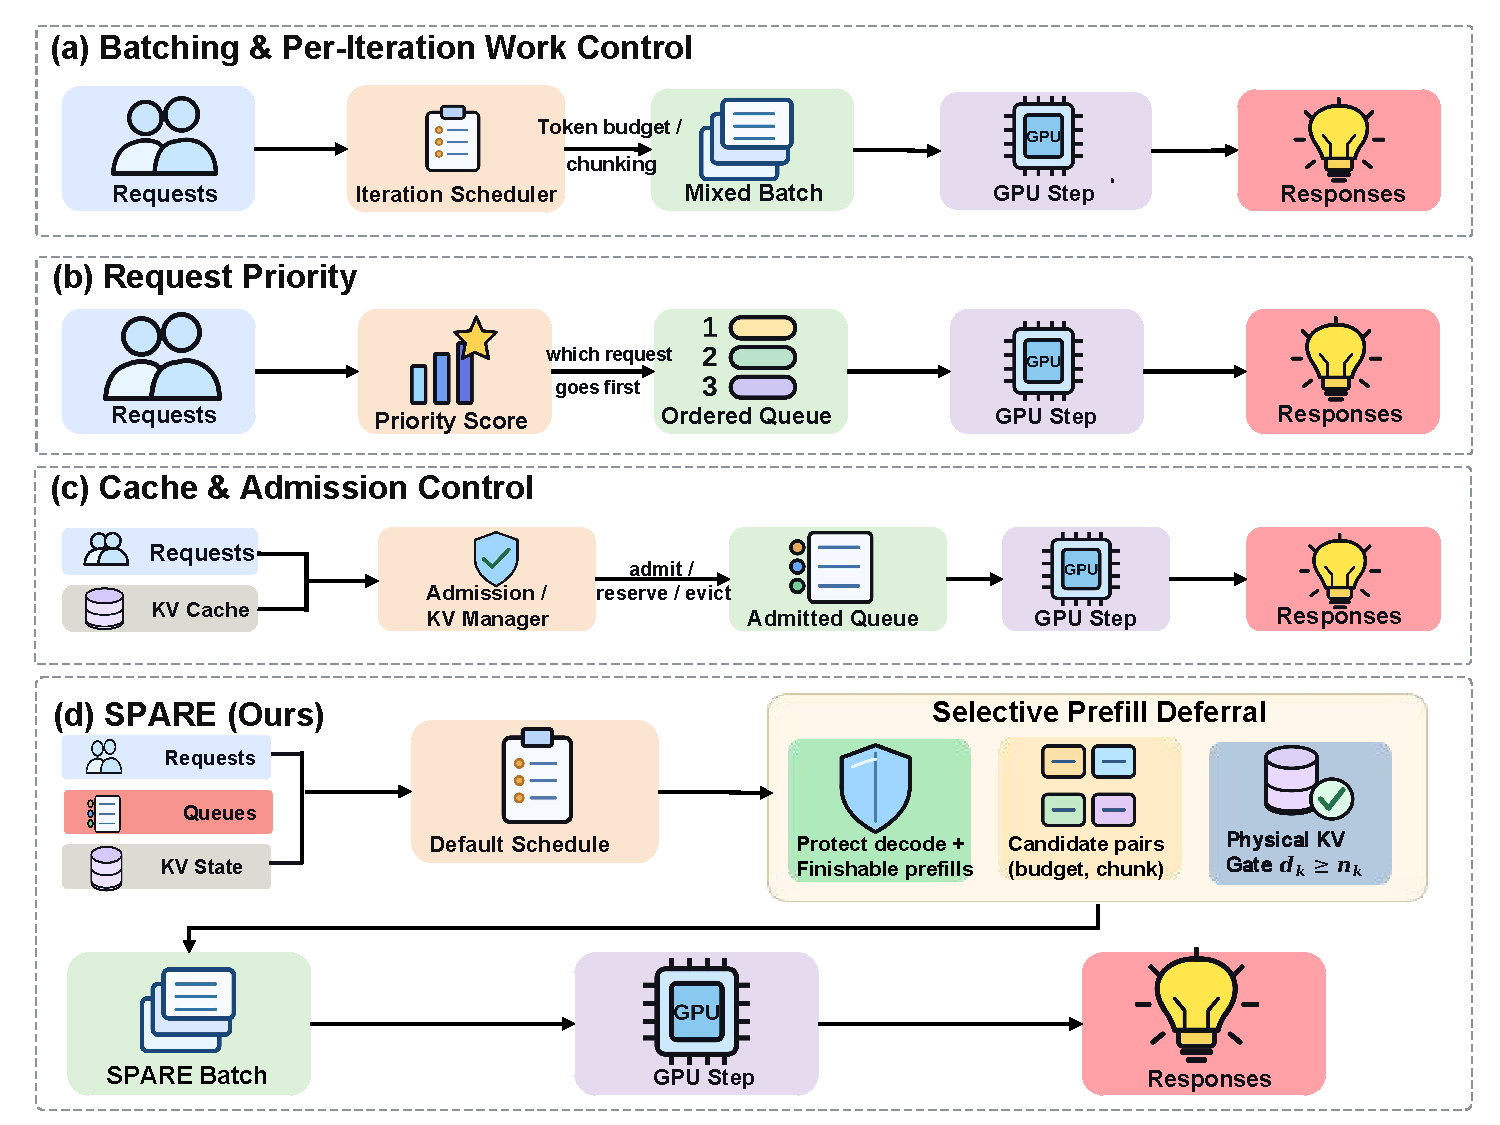
\includegraphics[width=\columnwidth]{figures/related.pdf}
\caption{Comparison of scheduling controls in LLM serving: (a) batching and per-iteration work control; (b) request priority; (c) cache and admission control; and (d) SPARE's selective prefill deferral.}
\label{fig:spare-comparison}
\end{figure}

To tackle these throughput, latency, and memory costs, existing LLM-serving methods optimize three closely related scheduling decisions~\cite{wu2026fastserve,sun2024llumnix,she2026plaserve}. First, batching and per-iteration work control. Orca and vLLM V1 schedule requests at iteration granularity, Sarathi-Serve chunks prefills to mitigate decode stalls, and SOLA adapts scheduling decisions to request and system state \cite{intro_orca,intro_vllm,intro_sarathi,intro_sola}. These mechanisms improve utilization and execution overlap, but a scheduled chunk that leaves a prefill unfinished can still retain KV blocks without producing a first response. Second, request priority. SSJF prioritizes requests using predicted output length, LTR learns length-based rankings, TRAIL estimates remaining length from model representations, TIE incorporates prediction uncertainty, and UniBoost adjusts priorities using runtime signals \cite{intro_ssjf,intro_ltr,intro_trail,intro_tie,intro_uniboost}. Such methods determine which requests should receive service earlier, but priority alone does not determine how much physical KV space an unfinished prefill should acquire in the current iteration. Third, cache and admission control. PagedAttention reduces memory fragmentation, S$^3$ uses length estimates for memory-aware scheduling, Past-Future anticipates future KV demand, KV-constrained online scheduling studies admission under memory limits, and Apt-Serve jointly considers cache management and adaptive scheduling \cite{intro_vllm,intro_s3,intro_pastfuture,intro_onlinekv,intro_aptserve}. These approaches improve memory allocation and admission decisions, yet requests that have already been admitted can continue expanding their KV occupancy before producing their first tokens.
A scheduler trained with reinforcement learning can also choose per-iteration actions, but its capacity advantage may diminish when the workload mix or cache budget differs from its training setting.

These advances establish batching, request priority, and admission as key scheduling decisions, while revealing an additional opportunity for controlling prefill progress at iteration granularity. Specifically, under a fixed request order, how much unfinished prefill should the scheduler advance in the current iteration? This decision cannot be made from token counts alone. Reducing a token allocation saves memory only when it crosses a physical KV-block boundary, whereas deferring a prefill that could finish in the current iteration directly postpones its first response. Moreover, the appropriate amount of deferral changes with available KV space, accumulated unfinished input, and incoming workload pressure~\cite{saemann2026ppas}. Effective progress control must therefore preserve immediate output opportunities while selectively suppressing prefill work whose current progress consumes scarce KV capacity without yet producing output.

Motivated by this observation, we propose SPARE, a KV-cache-aware online scheduler that selectively controls unfinished prefill progress using only observable runtime state. As illustrated in Figure~\ref{fig:spare-comparison}(d), SPARE first constructs a reference schedule using the default token budget and chunk limit with its established request order. It protects the reference allocations for normal decode work and for prefills that can finish and produce a first token in the current iteration. SPARE then evaluates alternative token budgets and chunk limits under the same request order, selecting a reduced schedule only when the protected work remains intact and the reduction saves sufficiently many \emph{physical} KV blocks. The required savings adapt to free cache space, unfinished input work, and recent arrivals, adjusting the deferral decision to current resource pressure while preserving immediate response opportunities.

We conduct extensive evaluations across diverse workloads and a wide range of KV-cache budgets. Experimental results demonstrate that SPARE outperforms the baseline schedulers, achieving up to 2.65$\times$ the serving capacity under latency and stability constraints and reducing mean TTFT by up to 82.1\% at matched arrival rates. Furthermore, SPARE reduces average request completion time by 19.5\%--41.1\% compared with 11 baseline schedulers in an overall-serving evaluation. Across four language models, simulator predictions and hardware serving runs agree on whether service requirements are met in 99.2\% of cases.

This paper makes three contributions. First, we identify \emph{per-iteration prefill progress} as a distinct scheduling dimension that couples immediate first-response opportunities with persistent KV-cache occupancy, extending scheduling control beyond request ordering, batching, and admission. Second, we develop SPARE, an online scheduler that combines selective prefill deferral, output protection, physical-block-aware savings, and pressure-adaptive control to improve latency-constrained serving capacity across diverse memory configurations. Third, we develop an extensible iteration-level evaluation framework that preserves vLLM V1 scheduling semantics and physical KV allocation while supporting interchangeable scheduling policies, workloads, execution-time models, and KV-cache budgets, and validate its predictions against GPU serving across multiple language models.


\section{Preliminaries}
\label{sec:preliminaries}

\subsection{Request Execution}
\label{sec:request-execution}

We study online scheduling within a single large language model (LLM) serving instance. The instance maintains request queues and an iterative scheduler; concurrent requests share its compute resources and key--value (KV) cache. Request $i$ arrives at time $r_i$ with $P_i$ input tokens. Its input length is known on arrival, while its final output length is revealed as generation proceeds.

Each request first undergoes \emph{prefill}, which processes the input and produces the first output token, followed by \emph{decode}, which generates subsequent tokens one at a time. Let $f_i$ be the time at which request $i$ receives its first token. Its time to first token (TTFT) is
\begin{equation}
    \mathrm{TTFT}_i = f_i-r_i.
    \label{eq:ttft}
\end{equation}
TTFT includes queueing, waits between prefill chunks, and the computation needed to produce the first token. In each iteration, the scheduler allocates tokens to running and waiting requests. A long prefill may span multiple iterations, and a batch may also contain decode work. Requests arriving during an iteration become eligible in a later iteration.

\subsection{KV-Cache Constraints and Recovery}
\label{sec:kv-constraints}

Requests retain the keys and values of processed tokens in the KV cache to reuse their computed context. We consider an instance with $C$ usable physical KV blocks, each holding the state of $B$ tokens. Blocks are allocated as needed, remain resident across iterations, and are released when a request completes. Independent requests do not share cached prefixes.

Let $\mathcal R_k$ denote the arrived, unfinished requests at the start of iteration $k$, and let $b_{i,k}$ be the number of blocks held by request $i$. The number of free blocks is
\begin{equation}
    F_k=C-\sum_{i\in\mathcal R_k} b_{i,k}.
    \label{eq:free-kv-blocks}
\end{equation}
A request can use free slots in blocks it already holds, so processing more tokens need not allocate more blocks. Scheduling is also constrained by the per-iteration token budget, per-request chunk limit, concurrency limit, and maximum context length. When KV space is insufficient, the engine may preempt a request and release its blocks. Resuming the request requires recomputing the released context, adding computation and waiting time.

Let $o_{i,k}$ be the number of output tokens already generated and $c_{i,k}$ the length of the computed context whose KV state remains resident. The work required before request $i$ produces its next output token is
\begin{equation}
    \ell_{i,k}=P_i+o_{i,k}-c_{i,k}.
    \label{eq:remaining-work}
\end{equation}
Normal decode has $\ell_{i,k}=1$. Preemption resets $c_{i,k}$ to zero while preserving the generated output, so recovery must reconstruct the released KV state. Online scheduling decisions use the states of arrived requests, the current queues and KV cache, and observed arrival history.

\subsection{Service Objectives: TTFT and Serving Capacity}
\label{sec:service-objectives}

We evaluate both first-response latency and the request rate sustained under latency constraints. Following prior SLO-aware serving evaluations~\cite{intro_sarathi,zhong2024distserve,patel2024splitwise}, we use \emph{serving capacity} as the throughput metric: the highest request arrival rate an instance can sustain while meeting its service requirements.

Fix a KV budget $C$, workload distribution $D$, and online scheduling policy $\pi$. The workload $D$ specifies request characteristics and the arrival process apart from its rate. Let $\lambda$ be the offered request arrival rate in queries per second (QPS). With $(\pi,C,D)$ fixed, let $L(\lambda)$ denote mean TTFT, $H(\lambda)$ the 99th-percentile time between consecutive output tokens (P99 TBT), and $\Delta(\lambda)$ the increase in unfinished requests over a measurement interval. Given a mean-TTFT limit $\theta$, a P99-TBT limit $H_{\max}$, and a backlog-growth limit $\Delta_{\max}(\lambda)$, serving capacity is
\begin{equation}
\begin{aligned}
\Lambda_{\pi,C,D}(\theta)=\sup\bigl(\{0\}\cup\{\lambda>0:\;
    &L(\lambda)\le\theta,\\
    &H(\lambda)\le H_{\max},\\
    &\Delta(\lambda)\le\Delta_{\max}(\lambda)\}\bigr).
\end{aligned}
\label{eq:serving-capacity}
\end{equation}

We seek lower mean TTFT at the same arrival rate and higher capacity under the same mean-TTFT limit. SPARE selects per-iteration progress from online state; $\theta$ specifies the capacity evaluation target. Section~\ref{sec:evaluation} describes the finite-window arrival-rate scan used to estimate capacity.

% Translation of SPARE_METHODOLOGY_CN_V6_ANNOTATED.md, with the two
% author-approved corrections dated 2026-10-20. Editorial notes are omitted.
% Prerequisites: amsmath, amssymb, booktabs, algorithm, algpseudocode.
% Request and KV notation follows the manuscript's Preliminaries.

\section{SPARE Design}
\label{sec:spare-design}

\subsection{Core Insight and Overview}
\label{sec:spare-overview}

In online LLM serving with a limited KV cache, advancing prefill as early as possible appears to bring requests closer to their first token. Yet computational progress does not always translate into lower mean TTFT. Advancing an unfinished prefill makes its KV states resident before it produces a first token. Under continued arrivals, these states occupy space needed by other requests and can trigger preemption and recomputation. The resulting waits for other requests can offset the benefit of advancing some requests early. SPARE therefore considers both immediate output opportunities and the persistent KV cost of advancing unfinished work.

SPARE uses this observation to selectively control computation in each round. For requests whose prefill can finish under the default plan, it preserves the token allocations needed to produce their first token. For requests in normal decode, it preserves their generation allocations so that they continue toward completion. Other work can be deferred when reducing the budget saves physical KV block allocations and meets the savings requirement under the current input pressure. SPARE thus preserves existing output opportunities while limiting unnecessary KV growth, leaving space for subsequent request admission and execution.

The serving configuration specifies a default total token budget $T$ and a per-request chunk limit $K$. In round $k$, SPARE selects positive integers $(T_k,K_k)$ such that $T_k\le T$ and $K_k\le\min\{K,T_k\}$. If request $i$ receives an allocation of $x_{i,k}$ tokens, then
\begin{equation}
\sum_{i\in\mathcal R_k}x_{i,k}\le T_k,
\qquad 0\le x_{i,k}\le\min\{\ell_{i,k},K_k\}.
\tag{4}\label{eq:spare-budget}
\end{equation}

Figure~\ref{fig:spare-architecture} summarizes SPARE's per-iteration
scheduling workflow. Output protection identifies the base plan's
allocations to preserve (Section~\ref{sec:spare-protection}). Free KV
space, unfinished input work, and recent arrivals determine the required
physical KV block savings (Section~\ref{sec:spare-preservation}). SPARE
projects candidate configurations under the same request state and order,
selects the first eligible configuration, and passes its token budget and
chunk limit to the native scheduler for execution
(Section~\ref{sec:spare-selection}).

\begin{figure}[htbp]
  \centering
  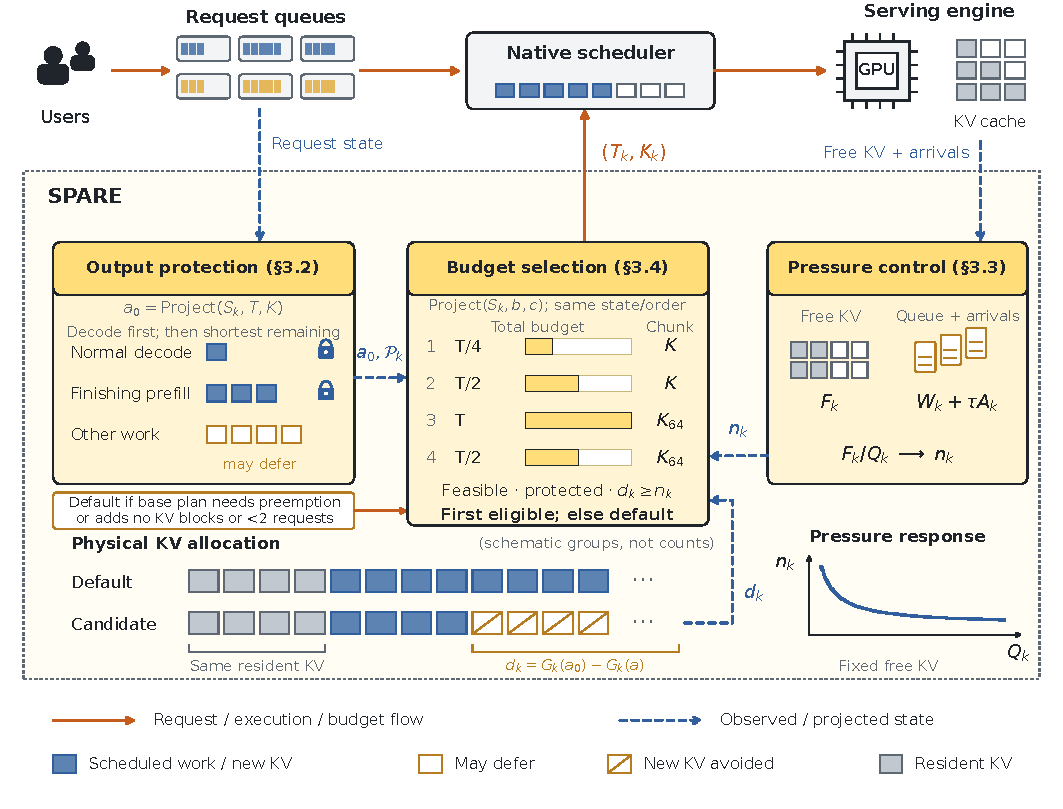
\includegraphics[width=\columnwidth]{figures/spare_architecture.pdf}
    \caption{SPARE scheduling architecture. KV block groups are
schematic; resident KV remains unchanged, and slashed cells
mark avoided new allocations.}
  \label{fig:spare-architecture}
  \Description{Runtime state feeds output protection and threshold
  computation. These feed candidate projection and selection, which
  determines the token budget and chunk limit for native execution.
  The updated state feeds the next iteration.}
\end{figure}


% Figure placeholder retained from the source; no figure asset was supplied.
% Suggested caption: Selective progress in SPARE. Token allocations are
% protected for prefill that can finish in the current round and for normal
% decode in the default plan. Budget reductions defer other work to reduce
% physical KV block allocations. Free space and input pressure determine the
% minimum required savings. Candidate projection combines output protection
% and space requirements into the round's budget decision. The figure should
% show how SPARE preserves current output opportunities and leaves KV space
% for subsequent admission and execution.

\subsection{Output-Aware Allocation Protection}
\label{sec:spare-protection}

Selective deferral first requires identifying the work that should continue in the current round. SPARE constructs a base plan $a_0$ using the default configuration $(T,K)$. The output opportunities already available in this plan determine which request allocations must be preserved when the budget is reduced.

The base plan prioritizes requests in normal decode in the running queue. The remaining running requests and the waiting requests are each ordered by increasing remaining work $\ell_{i,k}$, with earlier arrivals breaking ties. The scheduler processes the running queue before admitting waiting requests. The base plan and all candidates use this request priority; only the total budget and per-request chunk limit vary.

SPARE constructs $a_0$ through plan projection, $\operatorname{Project}(S_k,T,K)$, where $S_k$ contains the request and KV state collected for the current round. Projection estimates each request's token allocation and additional physical block demand in priority order, subject to limits on KV space, running concurrency, and model context length. The native scheduler performs the actual request and KV block allocation. If the base plan requires preempting a running request, SPARE retains the default configuration and leaves preemption and recovery to the native scheduling procedure. Otherwise, it uses the projected base plan for output protection and candidate evaluation. Appendix~\ref{app:spare-projection} gives the projection procedure.

Two types of allocations in the base plan provide output opportunities. For a request that has not produced its first token and can finish its remaining prefill in this round, preserving its allocation retains that first-token opportunity. For a request in normal decode, preserving its allocation maintains generation progress. Let $x_{i,k}(a)$ be the number of tokens allocated to request $i$ by plan $a$. SPARE defines the protected set as
\begin{equation}
\begin{aligned}
\mathcal P_k={}&\{i\in\mathcal R_k:x_{i,k}(a_0)>0,
\ o_{i,k}>0,\ \ell_{i,k}=1\}\\
&\cup\{i\in\mathcal R_k:x_{i,k}(a_0)>0,
\ o_{i,k}=0,\ x_{i,k}(a_0)=\ell_{i,k}\}.
\end{aligned}
\tag{5}\label{eq:spare-protected-set}
\end{equation}
A candidate plan $a$ must satisfy
\begin{equation}
x_{i,k}(a)\ge x_{i,k}(a_0),
\qquad \forall i\in\mathcal P_k.
\tag{6}\label{eq:spare-protection}
\end{equation}

This constraint preserves first-token opportunities for prefill that can finish and maintains generation in normal decode. Continued decoding also advances requests toward completion, when their KV blocks are released. Requests that have already produced output but require multiple tokens of recomputation participate in candidate projection according to their remaining work. With the protected allocations established, SPARE next determines whether deferring other work yields physical space savings.

\subsection{Pressure-Aware KV Space Preservation}
\label{sec:spare-preservation}

Reducing token allocations does not necessarily reduce KV occupancy because requests can use empty slots in physical blocks they already hold. SPARE therefore measures the direct space benefit of deferral by the number of physical KV block allocations saved relative to the base plan. For a plan $a$ that requires no preemption, the additional block demand is
\begin{equation}
\begin{aligned}
G_k(a)&=\sum_{i:x_{i,k}(a)>0}
\max\!\left\{0,
\left\lceil\frac{c_{i,k}+x_{i,k}(a)}{B}\right\rceil-b_{i,k}
\right\},\\
&\hspace{2em}G_k(a)\le F_k.
\end{aligned}
\tag{7}\label{eq:spare-block-demand}
\end{equation}
The block savings of a candidate plan are
\begin{equation}
d_k(a)=G_k(a_0)-G_k(a).
\tag{8}\label{eq:spare-block-savings}
\end{equation}

This measure follows the granularity of physical block allocation. If the deferred tokens would have occupied empty slots in blocks already held by a request, the corresponding block savings are zero. A budget reduction becomes acceptable to SPARE only when it yields sufficient physical block savings.

The required savings depend on current input pressure. When space is plentiful, there is less reason to defer computation to save a small number of KV blocks. As pending input accumulates and free space becomes scarce, preserving KV space becomes more valuable. SPARE therefore uses a state-dependent minimum block savings threshold $n_k$ and requires $d_k(a)\ge n_k$. To measure the pending input work of requests that have not produced their first token, we define
\begin{equation}
W_k=\sum_{i\in\mathcal R_k:o_{i,k}=0}
\max\{0,P_i-c_{i,k}\}.
\tag{9}\label{eq:spare-pending-work}
\end{equation}

$W_k$ includes both waiting requests and ongoing chunked prefill. Recent arrivals also contribute to KV demand. SPARE estimates the recent input rate from observed arrival events. If request $j$ arrives at time $s_j$ and the estimate is read at time $t_k$, then
\begin{equation}
A_k=\sum_{j:s_j\le t_k}\frac{P_j}{H}
\exp\!\left(-\frac{t_k-s_j}{H}\right),\qquad H>0.
\tag{10}\label{eq:spare-arrival-rate}
\end{equation}

$A_k$ is measured in tokens/s. The time scale $H$ controls how long recent arrivals influence the estimate, and the factor $1/H$ makes each request's rate contribution integrate to its input length (Appendix~\ref{app:spare-normalization}). SPARE uses a time scale $\tau\ge0$ to convert the recent rate into an input amount, combines it with $W_k$ as a short-term input pressure signal, and computes
\begin{equation}
\begin{aligned}
Q_k&=1+\frac{W_k+\tau A_k}{B},\\
n_k&=\min\!\left\{n_{\max},
\max\!\left\{1,
\left\lceil n_0+\alpha\frac{F_k}{Q_k}\right\rceil
\right\}\right\}.
\end{aligned}
\tag{11}\label{eq:spare-threshold}
\end{equation}

$Q_k$ expresses input pressure on a block-count scale, with the constant $1$ keeping the expression defined when there is no input work. As relative free space $F_k/Q_k$ increases, the minimum required savings rise. Higher input pressure makes smaller block savings acceptable. The parameters $n_0$ and $\alpha$ control the baseline requirement and its response to the state. We fix $n_0=8$, $\alpha=128$, $n_{\max}=100000$, and $H=\tau=1\,\mathrm{s}$. All candidates in a round share the same $n_k$.

\subsection{Online Budget Selection and Execution}
\label{sec:spare-selection}

Output protection identifies the computation that a budget reduction must preserve, while the block savings threshold determines when other work can be deferred. SPARE combines these requirements into an online decision by adjusting the total token budget and per-request chunk limit. Reducing the total budget limits overall progress in the round while allowing individual requests to receive larger chunks within the chunk limit. Lowering the chunk limit restricts each request's share of computation, allowing the budget to cover more requests. SPARE uses the four fixed, ordered candidates in Table~\ref{tab:spare-candidates} to cover these two controls and their combination.

\begin{table}[tbp]
\centering
\caption{SPARE's ordered candidate configurations. The effective chunk limit is the smaller of the listed limit and the candidate's total budget.}
\label{tab:spare-candidates}
\small
\begin{tabular}{@{}cllc@{}}
\toprule
Order & Total token budget & Chunk limit & $T=1024,\ K=256$ \\
\midrule
1 & $\max\{1,\lfloor T/4\rfloor\}$ & $K$ & $(256,256)$ \\
2 & $\max\{1,\lfloor T/2\rfloor\}$ & $K$ & $(512,256)$ \\
3 & $T$ & $\min\{64,K\}$ & $(1024,64)$ \\
4 & $\max\{1,\lfloor T/2\rfloor\}$ & $\min\{64,K\}$ & $(512,64)$ \\
\bottomrule
\end{tabular}
\end{table}

Candidates are evaluated in the order shown, first testing reductions in the total budget, then a lower chunk limit and its combination with a reduced total budget. Each candidate starts from the same request state and free block count for the round. The projection $\operatorname{Project}(S_k,b,c)$ estimates which requests would execute, their token allocations, and the additional KV block demand. SPARE retains the first candidate whose plan is nonempty and feasible, preserves the allocations required by Equation~\eqref{eq:spare-protection}, and satisfies $d_k(a)\ge n_k$. Acceptance also requires that the base plan allocate new KV blocks and that at least two requests remain unfinished. If none of the four candidates qualifies, SPARE uses the default configuration.

Algorithm~\ref{alg:spare-scheduling} summarizes the per-round decision. Candidate projection checks the resource allocation under a proposed configuration. After selection, the native scheduler uses the chosen budget to perform the actual allocation of requests, tokens, and KV blocks. If the base plan requires preemption, SPARE uses the default configuration and leaves preemption and recovery to the native scheduling procedure.

\begin{algorithm}[tbp]
\caption{SPARE Per-Iteration Scheduling}
\label{alg:spare-scheduling}
\begingroup
\algtext*{EndIf}
\small
\begin{algorithmic}[1]
\Require Current request and KV state, arrival-rate estimator, default configuration $(T,K)$
\Ensure Native scheduling result for the current round
\State Order the queues as in Section~\ref{sec:spare-protection}; collect state $S_k$
\State Update and read the recent input rate $A_k$
\State $a_0\gets\Call{Project}{S_k,T,K}$
\State Compute $W_k$, $Q_k$, and $n_k$ using Equations~\eqref{eq:spare-pending-work}--\eqref{eq:spare-threshold}
\State $(b^*,c^*,a^*)\gets(T,K,a_0)$; $\mathit{chosen}\gets\mathrm{false}$
\If{$a_0\ne\bot$}
    \State Construct $\mathcal P_k$ from $a_0$ using Equation~\eqref{eq:spare-protected-set}
    \For{$(b,c)$ in the order of Table~\ref{tab:spare-candidates}}
        \State $a\gets\Call{Project}{S_k,b,c}$
        \State \textbf{if} $a=\bot$ or $a$ is empty: \textbf{continue}
        \State $d\gets G_k(a_0)-G_k(a)$
        \State $\mathit{guard}\gets\bigl[\forall i\in\mathcal P_k:\ x_{i,k}(a)\ge x_{i,k}(a_0)\bigr]$
        \If{$\begin{aligned}[t]
            &\neg\mathit{chosen}\ \land\ \mathit{guard}\ \land\ d\ge n_k\\
            &\qquad\land\ G_k(a_0)>0\ \land\ |\mathcal R_k|\ge2
            \end{aligned}$}
            \State $(b^*,c^*,a^*)\gets(b,c,a)$
            \State $\mathit{chosen}\gets\mathrm{true}$
        \EndIf
    \EndFor
\EndIf
\State $\mathit{output}\gets\Call{NativeSchedule}{b^*,c^*}$
\State \Return $\mathit{output}$
\end{algorithmic}
\endgroup
\end{algorithm}

$\operatorname{Project}$ returns the projected token allocations and additional block demand; $\bot$ indicates that a running request would require preemption. Subsequent candidate evaluations leave the first selected configuration unchanged. The pair $(b,c)$ contains the raw candidate parameters; allocation uses $T_k=b$ and $K_k=\min\{b,c\}$. The procedure \textsc{NativeSchedule} calls the native scheduler with the selected configuration and restores the defaults afterward. Appendix~\ref{app:spare-projection} describes how the implementation checks consistency between a projected plan and the actual allocation.

Each decay or update of the arrival-rate estimate takes constant time. Let $m$ be the number of unfinished requests. Sorting takes $O(m\log m)$ time, and each plan projection takes $O(m)$ time. With four candidates, SPARE's scheduling decision takes $O(m\log m)$ time per round and uses $O(m)$ temporary space.


\section{Evaluation}
\label{sec:evaluation}

% Insert under the manuscript's existing Evaluation section.
\subsection{Experimental Setup}
\label{sec:setup}

\subsubsection{Environment.}
GPU experiments use Qwen2.5-7B-Instruct~\cite{spare_qwen} on an RTX 4090 (24~GB) with vLLM~0.9.2 V1~\cite{intro_vllm,vllmteam2025v1}.
Capacity sweeps and RL comparisons use our iteration-level simulator, which reuses V1 scheduling and paged KV allocation with execution times fitted to GPU measurements.
The default per-iteration token budget is $T=1024$, with a per-request chunk limit of $K=256$.
The main simulation sweep covers 27 configured KV sizes from 1,024 to 12,032 blocks, with 16 tokens per block; usable capacity $C$ excludes one reserved block.


\subsubsection{Datasets.}
We use the Azure Code and Conversation traces~\cite{spare_azure}.
Code has longer prompts and shorter outputs than Conversation. 
%across our test segments, their median prompt/output lengths are 1,981/8 and 873.5/40.5 tokens, respectively.
%We select intact requests with positive lengths, at most 512 output tokens, and at most 8,000 total tokens.
These bounds retain 99.64\% of Code and 96.62\% of Conversation requests in the original one-week traces; the total-length bound fits the shared 8,176-token context limit, while the output bound controls the cost of broad capacity scans.
Each workload provides 50 disjoint test segments of 64 length pairs from two dates.
Request streams sample intact pairs with Poisson arrivals.
Each run has 60~s of arrivals and 20~s of warm-up; requests arriving during 20--60~s are tracked through completion.
Compared methods receive identical request streams.

\subsubsection{Baselines.}
We compare scheduling policies on a common V1 backend in three groups:
(1)~\emph{Batch scheduling:} native vLLM V1 and the Sarathi rule~\cite{intro_sarathi}, which prioritizes decode and chunks prefill.
(2)~\emph{Admission and request ordering:} Orca reservation~\cite{intro_orca} and Past-Future~\cite{intro_pastfuture} use output bounds or estimates to control admission; the S$^3$ packing proxy~\cite{intro_s3} and LTR scoring proxy~\cite{intro_ltr} use estimated lengths to pack or rank requests.
(3)~\emph{State-aware scheduling:} the Apt-Serve KV rule~\cite{intro_aptserve} prioritizes requests by pending time per required block; SOLA~\cite{intro_sola} uses predicted latency pressure; the UniBoost rule~\cite{intro_uniboost} uses execution-phase signals to adjust priority.
Past-Future and SOLA each have two variants, giving 11 external baseline implementations.
We additionally compare an independent Double DQN that selects budgets and chunk limits with frozen evaluation weights.
SRP, which keeps SPARE's ordering and disables deferral, and fixed budgets of 256/512 tokens serve as controls.

\subsubsection{Metrics.}
Following Section~\ref{sec:service-objectives}, we sweep the mean-TTFT limit $\theta$ at each fixed KV configuration and estimate serving capacity through finite-window arrival-rate scans, with the TBT and backlog constraints held fixed.
Capacity estimates use metrics averaged over 50 test windows per workload; summary curves report the equal-weight mean of Code and Conversation capacities at each $\theta$.
We also compare mean TTFT at matched arrival rates and KV configurations.
Sampling, simulator calibration, baseline adaptations, and capacity-search details are given in Appendix~\ref{app:experimental-details}.


\subsection{Simulator Validation}
\label{sec:simulator-validation}

We implement the same scheduling and paged KV-cache management rules
as the GPU serving environment and calibrate model-specific GPU
execution times, enabling controlled comparisons between SPARE and
baseline schedulers. We validate the simulator through paired GPU
and simulator replays across four LLMs, multiple KV-cache budgets,
and scheduling policies. As shown in
Table~\ref{tab:simulator-validation}, the simulator agrees with GPU
execution on 99.24\% of serving-feasibility decisions, where a run is
feasible if it satisfies the latency and service-stability constraints.
The mean absolute relative errors for mean TTFT and P99 TBT are
12.63\% and 10.40\%, respectively. On the three additional LLMs,
SPARE achieves 98.53\% feasibility agreement, with mean TTFT and
P99 TBT errors of 9.39\% and 5.71\%. Furthermore, across eight
completed fine-grained capacity searches for SPARE, the predicted
serving-capacity lower bounds differ from GPU measurements by
3.37\% on average. These results support using the simulator to
evaluate SPARE's latency and serving-capacity benefits.


\begin{table}[t]
  \centering
  \caption{GPU--simulator validation across four LLMs. Feasibility
  match is the percentage of paired runs with identical GPU and
  simulator pass/fail decisions. Latency errors are mean absolute
  relative errors across the evaluated schedulers; capacity error is
  computed for SPARE only. Parentheses give the number of completed
  capacity comparisons.}
  \label{tab:simulator-validation}

  \footnotesize
  \setlength{\tabcolsep}{3pt}
  \renewcommand{\arraystretch}{1.15}

  \begin{tabular*}{\columnwidth}
    {@{\extracolsep{\fill}}lcccc@{}}
    \toprule
    Model &
    \shortstack{Feasibility\\match (\%)} &
    \shortstack{Mean TTFT\\error (\%)} &
    \shortstack{P99 TBT\\error (\%)} &
    \shortstack{SPARE cap.\\error (\%)} \\
    \midrule
    Qwen2.5-7B & 99.92 & 14.02 & 12.05 & 0.97 (3) \\
    Qwen2.5-3B & 95.14 & 13.81 & 6.69  & 9.72 (2) \\
    Qwen3-8B   & 97.30 & 5.27  & 3.85  & 0.14 (2) \\
    Mistral-7B & 99.26 & 6.29  & 5.76  & 4.32 (1) \\
    \midrule
    \textbf{Overall}
    & \textbf{99.24}
    & \textbf{12.63}
    & \textbf{10.40}
    & \textbf{3.37 (8)} \\
    \bottomrule
  \end{tabular*}
\end{table}


\subsection{Main Results}
\label{sec:overall}

%The experimental results demonstrate that SPARE achieves a favorable capacity--latency trade-off across different KV-cache configurations and workloads, while also improving overall serving performance. We highlight three key findings below.

\subsubsection{Higher serving capacity across KV-cache budgets.}
As shown in Figure~\ref{fig:main-results-capacity}, SPARE achieves a more favorable capacity--latency trade-off than the baseline schedulers across a wide range of KV-cache configurations. For example, under a 4-second mean TTFT constraint, SPARE consistently outperforms the strongest baseline at each KV-cache budget, achieving an average capacity improvement of 14.8\% and a maximum gain of 25.6\%. 
%If this 14.8\% capacity gain were sustained for a comparable workload on a fixed-load fleet of 1,000 H100s, approximately 129 fewer GPUs would be needed, corresponding to US\$2.25 million in annual rental-equivalent costs at the same price.
Moreover, this advantage persists across a wide range of memory configurations, underscoring the robustness of SPARE under varying KV-cache constraints.

\begin{figure*}[htbp]
  \centering
  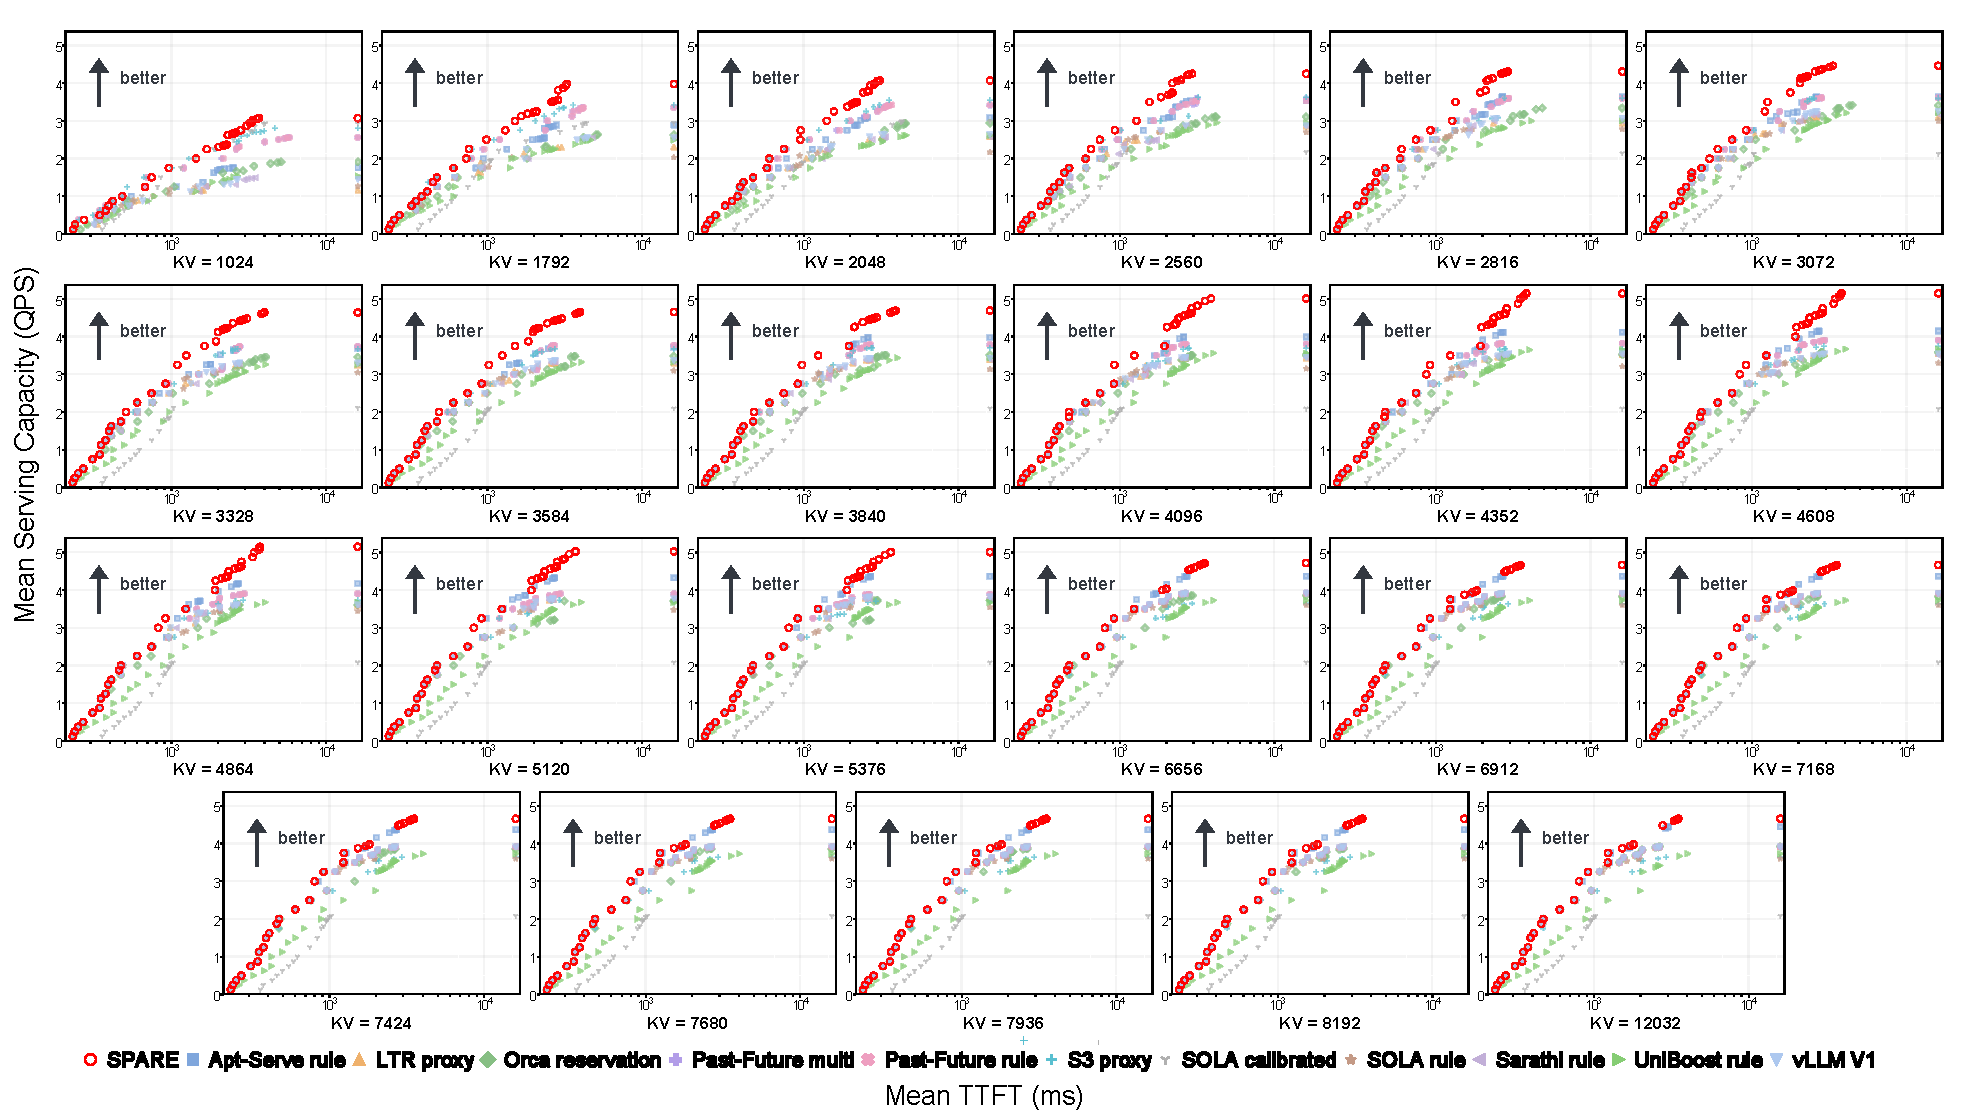
\includegraphics[width=\textwidth]{figures/main_results/figure1_for_mainresults_cropped.pdf}
  \caption{Capacity--latency trade-off across 23 KV-cache budgets. Each panel fixes a KV budget; curves farther up and left indicate better performance.}
  \label{fig:main-results-capacity}
\end{figure*}

\subsubsection{Lower mean TTFT at matched arrival rates.}

As shown in Figure~\ref{fig:main-results-matched}, SPARE consistently achieves the lowest mean TTFT across varying request arrival rates for both Code and Conversation workloads. While different schedulers exhibit comparable latency at low arrival rates, SPARE's advantage becomes increasingly pronounced as the request rate increases. At 3 QPS and 2,048 KV blocks, SPARE reduces mean TTFT by 23.6\%--66.7\% across Code and Conversation relative to the evaluated baselines meeting the TBT and backlog constraints. These results demonstrate SPARE's effectiveness in maintaining low initial response latency under increasing request demands across different workloads.

\begin{figure}[!t]
  \centering
  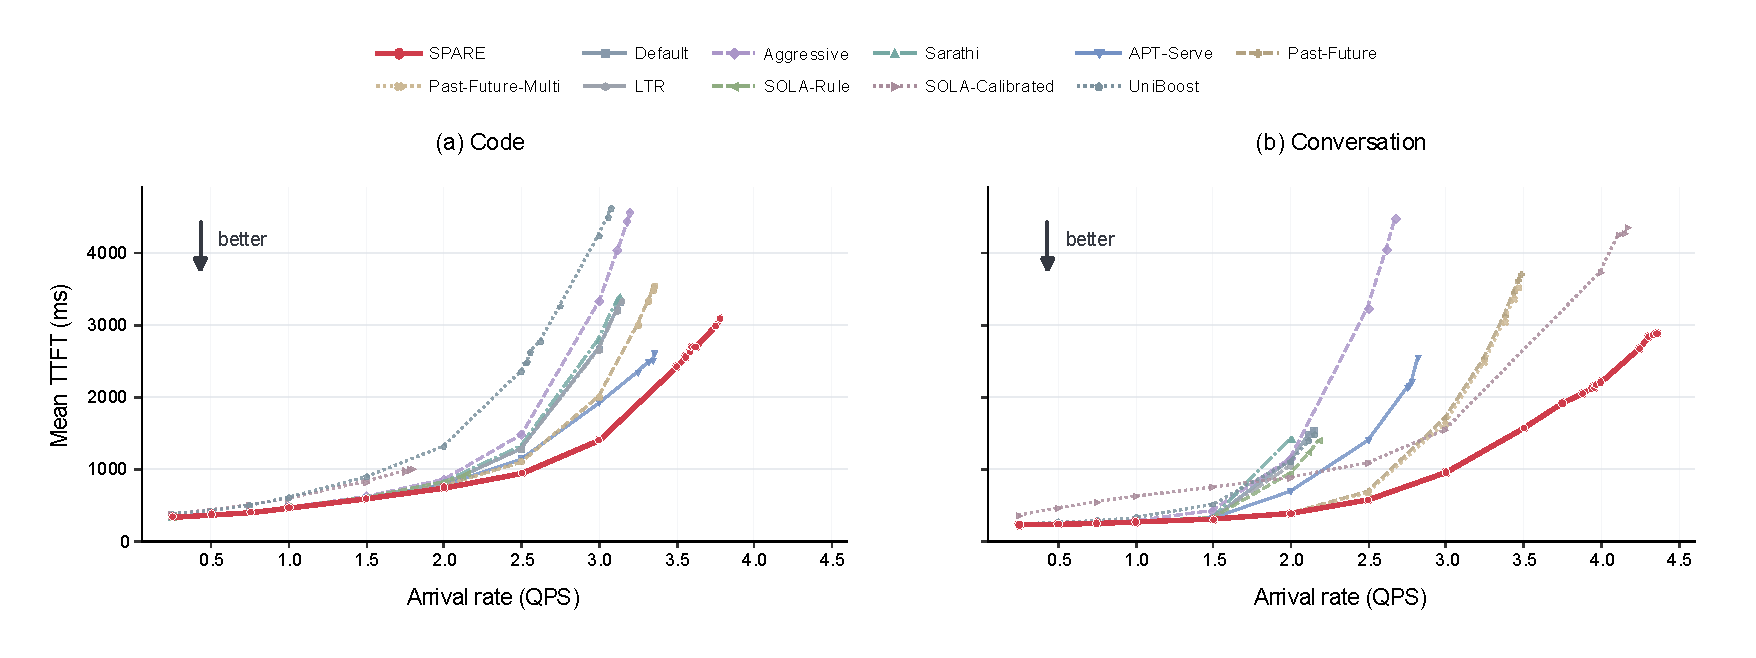
\includegraphics[width=\columnwidth]{figures/main_results/mainresults2_cropped.pdf}
  \caption{Mean TTFT by arrival rate for (a) Code and (b) Conversation; lower is better.}
  \label{fig:main-results-matched}
\end{figure}

\subsubsection{Improvements in overall serving performance.}

Beyond reducing mean TTFT, SPARE also delivers benefits in request completion latency and service quality. As shown in Table~\ref{tab:main-results-service}, SPARE achieves the lowest mean end-to-end latency of 3.64 s, outperforming the next-best baseline by 19.5\%. Moreover, SPARE attains the highest SLO attainment of 92.64\%, exceeding the strongest baseline by 2.95 percentage points. SPARE also achieves lower mean TBT than 10 of the 11 baselines and reduces preemptions by 84.7\% compared with vLLM V1. These results demonstrate that SPARE's advantages extend beyond initial response latency, enabling faster request completion, improved service-level compliance, and reduced preemption overhead.

\begin{table}[!t]
\caption{Overall serving performance. Bold marks the best value and underlining the second-best distinct value in each column; ties share
ranks. E2E: end-to-end latency; SLO: service-level objective;
LTR: learning to rank. Preemptions are counted per measurement window.}
  \label{tab:main-results-service}
  \centering
  \scriptsize
  \setlength{\tabcolsep}{1.5pt}
  \resizebox{\columnwidth}{!}{%
  \begin{tabular}{@{}lrrrrr@{}}
    \toprule
    Scheduler & \shortstack{TTFT mean\\(s)$\downarrow$} & \shortstack{E2E mean\\(s)$\downarrow$} & \shortstack{TBT mean\\(ms)$\downarrow$} & \shortstack{SLO attainment\\(\%)$\uparrow$} & \shortstack{Preemptions\\per window $\downarrow$} \\
    \midrule
    \textbf{SPARE} & \textbf{1.57} & \textbf{3.64} & \underline{46.92} & \textbf{92.64} & 9.18 \\
    vLLM V1 & 3.13 & 5.93 & 62.54 & 74.02 & 59.84 \\
    Sarathi rule & 3.22 & 6.02 & 62.39 & 77.39 & 57.69 \\
    Past-Future rule & 2.54 & 4.68 & 52.25 & 81.84 & 0.41 \\
    Past-Future multi & 2.54 & 4.67 & 52.18 & 81.98 & 0.27 \\
    Orca reservation & 4.34 & 5.97 & \textbf{40.55} & 61.78 & \textbf{0.00} \\
    S3 packing proxy & 2.45 & \underline{4.52} & 50.41 & 83.59 & \textbf{0.00} \\
    LTR score proxy & 2.94 & 6.04 & 65.57 & 73.62 & 59.04 \\
    Apt-Serve KV rule & \underline{2.01} & 4.85 & 64.75 & \underline{89.69} & 50.22 \\
    SOLA risk rule & 3.04 & 6.17 & 72.19 & 51.53 & 60.18 \\
    SOLA calibrated & 3.83 & 6.19 & 66.30 & 32.58 & \underline{0.24} \\
    UniBoost rule & 2.67 & 6.07 & 72.36 & 84.39 & 111.65 \\
    \bottomrule
  \end{tabular}
  }
\end{table}

\subsection{Ablation Study}
\label{sec:ablation}

We ablate three components on Conversation. \textbf{(1) w/o Deferral} retains SPARE's request ordering but disables selective prefill deferral (SRP). \textbf{(2) w/o Adaptive Threshold} fixes the savings threshold at $n=8$. \textbf{(3) w/o Arrival Extrapolation} sets $\tau=0$, removing arrival-rate extrapolation from the threshold. Both threshold variants use SPARE's candidate configurations, physical block-savings checks, and output protection.
Appendix~\ref{app:output-protection} evaluates output protection separately.


\begin{figure}[htbp]
\centering
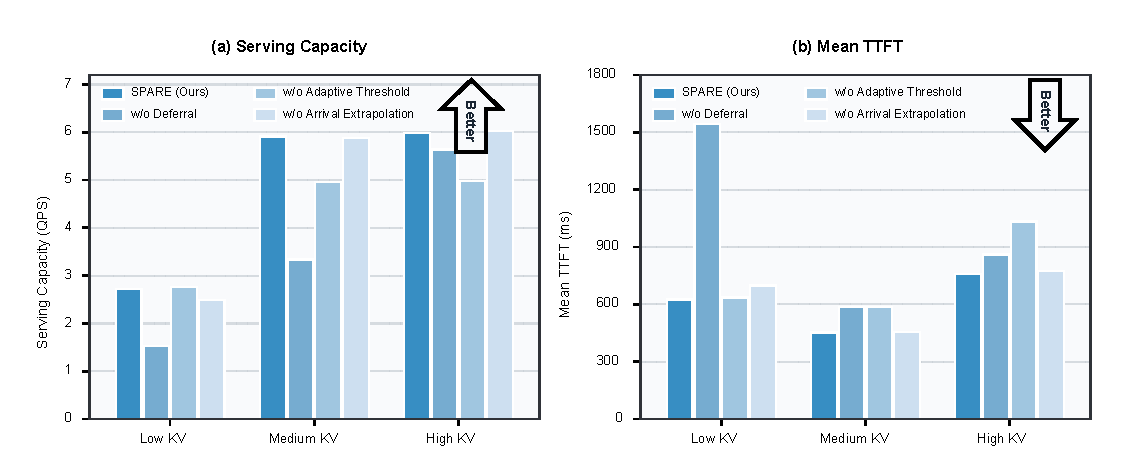
\includegraphics[width=\columnwidth]{figures/ablation_cropped.pdf}
\caption{(a) Serving capacity under a 4-s mean-TTFT limit and
common TBT/backlog constraints. (b) Mean TTFT at 1.5/3/4 QPS
for low/medium/high KV, respectively: the highest available
coarse-scan rate within all four variants' capacities at each KV budget.}
\label{fig:ablation}
\end{figure}

Figure~\ref{fig:ablation} shows that, relative to w/o Deferral, SPARE increases serving capacity by 78.9\% at low KV and 76.9\% at medium KV, compared with 6.0\% at high KV. Without deferral, low-KV mean TTFT also reaches 2.47$\times$ SPARE's, indicating that selective deferral limits premature KV growth and contention from prefills that cannot produce output immediately.
With deferral in place, threshold adaptation avoids delaying prefills for small block savings when KV headroom is ample. At high KV, fixing $n=8$ lowers capacity by 16.7\% and raises mean TTFT by 35.9\%. At low KV, the fixed threshold performs similarly to SPARE.
At the other end of the KV range, arrival extrapolation helps SPARE respond to growing demand. At low KV, setting $\tau=0$ lowers capacity by 8.5\% and raises mean TTFT by 11.7\%. Recent input rates let SPARE lower its savings threshold before new prefills expand KV demand. At medium and high KV, the capacity and mean-TTFT differences are small.

\subsection{Comparison with Reinforcement Learning}
\label{sec:rl-comparison}

We compare SPARE with a reinforcement learning (RL) scheduler
based on an independently trained Double DQN~\cite{rl_double_dqn}.
The RL policy is trained through online interaction with the
simulator on Conversation with 2,048 KV blocks, learning to
select the token budget and chunk limit based on the current
request and KV-cache state. During evaluation, its weights
remain frozen while it makes online scheduling decisions
across different workload distributions and KV-cache budgets
(Appendix~\ref{app:experimental-rl}).

As shown in Figure~\ref{fig:rl-comparison}(a), SPARE achieves
94.0\%--100.5\% of RL's serving capacity across the feasible
mean-TTFT limits without policy training.
However, as the workload shifts from Conversation to Code,
RL's capacity gain over SPARE drops from +4.69\% to $-5.16\%$
(Figure~\ref{fig:rl-comparison}(b)), indicating limited
generalization across workload distributions.
Similarly, as the KV-cache budget increases beyond the
training configuration, RL's relative advantage
diminishes and eventually reverses, with SPARE achieving
6.5\% higher capacity at 6,144 blocks
(Figure~\ref{fig:rl-comparison}(c)).
These results demonstrate that SPARE achieves competitive
performance without policy training while remaining effective
under changing workload and memory conditions.

\begin{figure}[htbp]
\centering
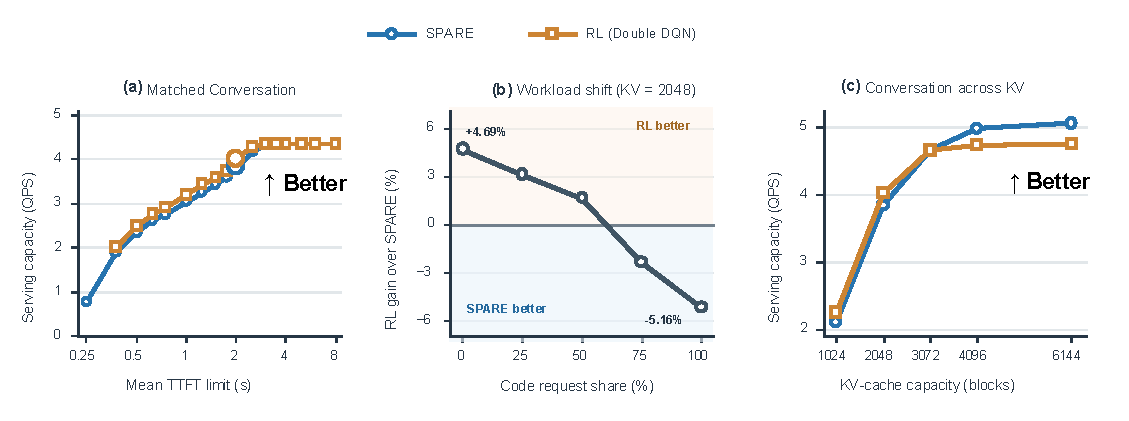
\includegraphics[width=\columnwidth]{figures/evaluation/rlresult_cropped .pdf}
\caption{Comparison of SPARE and RL.
(a) Serving capacity across mean-TTFT limits.
(b) RL capacity gain over SPARE under varying workload mixtures.
(c) Serving capacity across KV-cache budgets on Conversation.
Panels (b) and (c) use a 2-s mean-TTFT limit.}
\label{fig:rl-comparison}
\end{figure}

\subsection{Parameter Sensitivity}
\label{sec:parameter-sensitivity}

We examine the sensitivity of SPARE by halving or doubling
each parameter around the defaults $n_0=8$, $\alpha=128$,
and $H=\tau=1$~s. As shown in
Table~\ref{tab:parameter-sensitivity-main}, parameter
sensitivity is closely tied to KV-cache pressure.
Under tight memory budgets, overly restrictive
block-savings thresholds can suppress beneficial
prefill deferral, reducing both serving capacity and
latency performance. However, relaxing these thresholds
does not consistently improve performance across
workloads, indicating that effective scheduling requires
selective deferral rather than simply deferring more
prefills.

The results also show that $H$ and $\tau$ generally
have less influence than the threshold parameters
$n_0$ and $\alpha$, suggesting that SPARE's effectiveness
depends more on identifying worthwhile KV savings than
on precise arrival extrapolation. Moreover, parameter
sensitivity diminishes as KV-cache pressure decreases
in the Conversation workload. These findings support
using a unified default configuration without
workload-specific tuning. Complete results across
three KV budgets and both latency limits are reported
in Appendix~\ref{app:parameter-sensitivity}.


\begin{table}[t]
\centering
\caption{Parameter sensitivity at 1,024 KV blocks.
C is serving capacity (QPS) under a 2-s mean-TTFT
limit; L is mean TTFT (ms) at 2 QPS.
Bold indicates the default setting.}
\label{tab:parameter-sensitivity-main}

\vspace{3pt}
\small
\renewcommand{\arraystretch}{1.10}
\setlength{\tabcolsep}{3pt}

\resizebox{\columnwidth}{!}{%
\begin{tabular}{@{}lrr@{\hspace{8pt}}lrr@{}}
\multicolumn{3}{c}{\textbf{(a) Code}} &
\multicolumn{3}{c}{\textbf{(b) Conversation}} \\
\cmidrule(lr){1-3}\cmidrule(lr){4-6}
Setting & C$\uparrow$ & L$\downarrow$ &
Setting & C$\uparrow$ & L$\downarrow$ \\
\cmidrule(lr){1-3}\cmidrule(lr){4-6}

\textbf{Default} & \textbf{2.86} & \textbf{942.7} &
\textbf{Default} & \textbf{2.20} & \textbf{1511.3} \\

$n_0=4$ & 2.84 & 929.3 &
$n_0=4$ & 2.24 & 1395.4 \\

$n_0=16$ & 2.80 & 983.9 &
$n_0=16$ & 2.04 & 1849.9 \\

$\alpha=64$ & 2.92 & 941.8 &
$\alpha=64$ & 2.30 & 1362.2 \\

$\alpha=256$ & 2.82 & 1030.0 &
$\alpha=256$ & 2.08 & 1818.7 \\

\cmidrule(lr){1-3}\cmidrule(lr){4-6}
\end{tabular}%
}
\end{table}
\section{Related Work}
\label{sec:related-work}

Early model-serving systems developed adaptive batching, GPU sharing, and predictable latency~\cite{rw_clipper2017,rw_nexus2019,rw_clockwork2020,rw_infaas2021}. Autoregressive serving then introduced iteration-level batching and paged KV allocation~\cite{intro_orca,intro_vllm}. Sarathi-Serve used chunked prefill to reduce decode interference, FastServe explored preemption, and phase-disaggregated systems separated prefill from decode~\cite{intro_sarathi,wu2026fastserve,patel2024splitwise,zhong2024distserve}. These advances improve execution efficiency, but unfinished prefills can still retain KV blocks before generating their first tokens.

Other schedulers use predicted lengths or runtime signals to prioritize requests~\cite{intro_ltr,intro_trail,intro_tie,intro_uniboost}, or improve KV efficiency through packing, prediction, admission, or allocation~\cite{intro_s3,intro_pastfuture,intro_aptserve,intro_onlinekv,rw_vattention2025}. SOLA and P-PAS adapt execution decisions or token budgets based on serving state~\cite{intro_sola,saemann2026ppas}. Yet request ordering, admission, and budget adaptation do not by themselves determine whether partial prefill progress justifies new physical KV blocks while preserving immediate output opportunities. SPARE instead evaluates projected block savings under current input pressure and protects normal decode and prefills that can finish in the current iteration.


\section{Conclusion}

In this paper, we present SPARE, a KV-cache-aware online scheduler for improving serving capacity and latency in memory-constrained LLM serving. Unlike existing approaches that primarily optimize batching, request priority, or admission, SPARE treats per-iteration prefill progress as an additional scheduling dimension. We find that aggressively advancing an unfinished prefill is not always beneficial because it can consume persistent KV-cache space before producing an output, increasing contention and potentially triggering costly preemption and recomputation. Based on this observation, SPARE selectively defers unfinished prefill work when doing so yields sufficient physical KV-block savings, while preserving normal decode progress and prefills that can complete in the current iteration. Through extensive experiments across diverse workloads and KV-cache configurations, SPARE substantially improves serving capacity under latency constraints and effectively reduces mean TTFT at matched arrival rates. It also improves overall serving performance and remains competitive with a trained RL scheduler without requiring policy training, while the RL scheduler's advantage diminishes as the workload distribution and KV-cache budget shift away from its training configuration. What‘s more, we further develop and validate an iteration-level simulator that closely reproduces GPU serving behavior and enables controlled evaluation across scheduling policies and memory configurations.

In future work, we plan to extend progress-aware scheduling to more complex serving environments, including joint scheduling across multiple LLMs and disaggregated serving systems. A promising direction is to coordinate request routing, prefill progress, and resource allocation across heterogeneous models, enabling the serving system to adapt scheduling decisions to both workload characteristics and model-specific resource conditions.


\bibliographystyle{ACM-Reference-Format}
\bibliography{references}
\appendix
% Input after \appendix in the host manuscript.
\section{Supporting Scheduling Details}
\label{app:spare-details}

\subsection{Plan Projection and Execution}
\label{app:spare-projection}

$S_k$ contains the running and waiting requests ordered as in Section~\ref{sec:spare-protection}, each request's computed prefix length and held KV block count, and the free block count $F_k$. Projection also uses the block size $B$, the running concurrency limit $M$, and the context length limit $L$. It returns a projected plan $a=(x,G)$.

\paragraph{Projection procedure $\operatorname{Project}(S_k,b,c)$.}
\begingroup
\algtext*{EndFor}
\small
\begin{algorithmic}[1]
\State Initialize all $x_i\gets0$ and the total additional block demand $G\gets0$
\State $u\gets b$; $f\gets F_k$; $r\gets$ number of requests in the running queue
\For{each running request, then each waiting request, in priority order}
    \State \textbf{if} $u\le0$: \textbf{break}
    \State \textbf{if} $i$ is waiting and $r\ge M$: \textbf{break}
    \State $x\gets\min\{\ell_{i,k},c,u\}$
    \Statex \hspace{\algorithmicindent}\textbf{if} $i$ is running: $x\gets\min\{x,L-1-c_{i,k}\}$
    \State \textbf{if} $x\le0$: \textbf{continue}
    \State $g\gets\max\{0,\lceil(c_{i,k}+x)/B\rceil-b_{i,k}\}$
    \State \textbf{if} $g>f$ and $i$ is running: \Return $\bot$
    \State \textbf{if} $g>f$ and $i$ is waiting: \textbf{break}
    \State $x_i\gets x$; $u\gets u-x$; $f\gets f-g$; $G\gets G+g$
    \State \textbf{if} $i$ is waiting: $r\gets r+1$
\EndFor
\State \Return projected plan $a=(x,G)$
\end{algorithmic}
\endgroup

If a running request needs more additional KV blocks than remain free, projection returns $\bot$. If a waiting request cannot be admitted, projection retains the plan constructed so far and stops admitting requests. All candidates are projected from the same initial state for the round, and projection itself leaves the actual KV allocation unchanged.

The default implementation continues projecting the remaining candidates after recording the first qualifying candidate to collect diagnostic data, while retaining the selected configuration. The native \texttt{Scheduler.schedule()} performs the actual allocation. The implementation temporarily sets the total budget and chunk limit before the call and restores the defaults in a \texttt{finally} block. When the selected plan can be projected, it also verifies that the actual token allocations and additional block demand match the projection and that no preemption occurs. These checks leave the candidate acceptance rule unchanged.

\subsection{Time Normalization of the Arrival-Rate Estimate}
\label{app:spare-normalization}

In Equation~\eqref{eq:spare-arrival-rate}, $H>0$ is the decay time scale. The exponential kernel integrates to $H$, so the factor $1/H$ normalizes each request's rate contribution. For a request with input length $P_j$,
\begin{equation*}
\int_{s_j}^{\infty}\frac{P_j}{H}
\exp\!\left(-\frac{t-s_j}{H}\right)\,\mathrm dt=P_j.
\end{equation*}
Thus, $A_k$ has units of tokens/s, and its integral preserves the total number of input tokens while the rate reflects both recent arrival counts and input lengths. The implementation initializes the estimate to zero. After an elapsed interval $\Delta t$, it multiplies the current value by $e^{-\Delta t/H}$; on receiving a request with input length $P_j$, it adds $P_j/H$. The quantity $W_k+\tau A_k$ combines unfinished input work and recent arrivals into a short-term input pressure signal.

% Insert after the manuscript has entered appendix mode; do not add a second \appendix.
\section{Experimental Details}
\label{app:experimental-details}


\subsection{Execution configuration and simulator}
\label{app:experimental-simulator}

GPU measurements use FP16 and single-GPU eager execution. Chunked prefill is enabled; prefix caching and speculative decoding are disabled. The default running concurrency is 32 and the maximum model context length in the main simulator is 8,176 tokens. Each physical KV block holds 16 token positions. The engine reserves one block, so usable capacity is one block below the reported configured count. The token budget $T$ and chunk limit $K$ apply separately in each scheduling iteration; KV states persist across iterations until completion or preemption.

The simulator executes the V1 scheduling and allocation logic on CPU, including request admission, per-iteration token allocation, preemption, recomputation, and KV release. It advances the clock with a nonnegative affine timing model fitted to measured GPU iteration times. The features are a constant term, prefill token count, prefill attention work, decode request count, accumulated decode context length, the number of 256-token tiles, and indicators for prefill and mixed batches. For a prefill chunk of $n$ tokens following $c$ cached tokens, the attention-work term is $nc+n(n+1)/2$. Features are scaled before fitting by nonnegative least squares.

The frozen timing profile uses 25,747 iterations from 48 GPU runs of SPARE, SRP, and native V1 on the calibration cohort. The target is measured engine-step wall time, including instrumentation. Timing validation uses a separate cohort with disjoint request identities, and the main test inputs are also checked against calibration request identities. The simulated clock uses the fitted batch costs; policy-specific CPU decision time, including RL inference time, is not added to that clock. Direct scheduling-time measurements are reported with their measurement scope.

GPU replay constructs repeated-token prompts with the selected input lengths and fixes generation to the selected output lengths. Paired simulator/GPU comparisons use matching request arrivals, lengths, KV capacities, and policy configurations.
% ADDED CITATIONS: spare_qwen, yang2025qwen3, jiang2023mistral.
For Qwen2.5-3B, Qwen3-8B, and Mistral-7B~\cite{spare_qwen,yang2025qwen3,jiang2023mistral}, we fit the same timing-model features separately to GPU iterations from a pilot window of each workload, then freeze each profile before replaying four disjoint windows per workload. The cross-model validation compares SPARE, SRP, and Sarathi under model-specific KV-block settings; the scheduler and replay procedure are shared across models.

The Qwen2.5-7B aggregate in Table~\ref{tab:simulator-validation} covers SPARE, native V1, Sarathi, Past-Future, S$^3$, UniBoost, and Apt-Serve. 

\subsection{Dataset construction and measurement protocol}
\label{app:experimental-protocol}

The one-week Azure traces contain 16,803,695 Code and 27,303,999 Conversation requests. The filters in Section~\ref{sec:setup} retain 16,743,157 and 26,380,101 intact requests, respectively. Median prompt/output lengths in the 3,200 test requests per workload are 1,981/8 tokens for Code and 873.5/40.5 for Conversation.

Each workload uses 25 segments from each of two dates. Starting 512 eligible requests after each date anchor, we alternate taking and skipping 64 requests. An earlier date supplies 20 development segments and initial output-length history; their identities are disjoint from the test set. Each replay samples intact pairs with replacement from its segment's 64-request pool and draws exponential interarrival times. Seeds are fixed by segment, streams are shared across policies, and changing QPS rescales arrival intervals. Length-history updates use completed requests.

Arrivals span 0--60~s; requests arriving during 20--60~s are followed through completion for mean TTFT. Each run's P99 TBT pools their valid consecutive-token intervals. Backlog growth is the unfinished-request count at 60~s minus that at 40~s. Metrics are averaged equally over the 50 segments, so the TBT criterion applies to mean per-window P99. Every replay must be valid for a rate to pass.

Configured KV counts are 1,024, 1,792, 2,048, 2,560, then every 256 blocks through 8,192, plus 12,032. For each mean-TTFT limit $\theta$ in 0.25--16~s, passing rates must also meet P99 TBT $\le200$~ms and mean backlog growth $\le\max(2,\lambda)$, with $\lambda$ in QPS. We refine the contiguous passing region from low rates to a 0.01--0.02-QPS passing--failing bracket, stopping at the first observed failure and retaining local nonmonotonic observations. Bracket width measures search resolution. Horizontal plot extensions retain the last measured capacity and are marked in source data.

Summary curves plot the mean-TTFT limit against the equal-weight mean of independently estimated Code and Conversation capacities. Attained TTFT can differ between workloads and is recorded separately; breakpoints occur at measured TTFT values where capacity increases.

\subsection{Parameter sensitivity}
\label{app:parameter-sensitivity}

Table~\ref{tab:parameter-sensitivity-full} reports the one-at-a-time sweep over 24 paired windows per workload, drawn from the 50-window main evaluation. Each parameter is halved or doubled around its default. All settings share the same 2-QPS streams for mean TTFT; capacity is scanned separately under 2-s and 4-s mean-TTFT limits, mean window P99 TBT $\le200$~ms, and mean backlog growth $\le\max(2,\lambda)$. Capacity brackets are 0.01--0.02 QPS wide, describing search resolution.

\begin{table*}[t]
\centering
\small
\setlength{\tabcolsep}{4pt}
\caption{Parameter sensitivity. $C_2$/$C_4$: capacity (QPS) at 2-s/4-s mean-TTFT limits; $L$: mean TTFT (ms) at 2 QPS.}
\label{tab:parameter-sensitivity-full}
\begin{tabular*}{0.90\textwidth}{@{\extracolsep{\fill}}lrrrrrrrrr@{}}
\toprule
& \multicolumn{3}{c}{KV=1,024} & \multicolumn{3}{c}{KV=2,048} & \multicolumn{3}{c}{KV=4,096} \\
Setting & $C_2$ & $C_4$ & $L$ & $C_2$ & $C_4$ & $L$ & $C_2$ & $C_4$ & $L$ \\
\midrule
\multicolumn{10}{@{}l}{\textit{Code}} \\
\textbf{Default} & 2.86 & 3.36 & 942.7 & 3.38 & 3.46 & 738.9 & 3.54 & 3.76 & 733.7 \\
$n_0=4$ & 2.84 & 3.36 & 929.3 & 3.35 & 3.46 & 739.0 & 3.54 & 3.76 & 733.7 \\
$n_0=16$ & 2.80 & 3.10 & 983.9 & 3.41 & 3.56 & 734.9 & 3.54 & 4.14 & 733.7 \\
$\alpha=64$ & 2.92 & 3.38 & 941.8 & 3.22 & 3.22 & 742.0 & 3.47 & 3.54 & 733.7 \\
$\alpha=256$ & 2.82 & 3.40 & 1030.0 & 3.46 & 3.60 & 737.0 & 3.56 & 3.60 & 733.7 \\
$H=0.5$ s & 2.86 & 3.20 & 943.0 & 3.36 & 3.56 & 734.5 & 3.54 & 3.78 & 733.7 \\
$H=2$ s & 2.88 & 3.41 & 917.9 & 3.36 & 3.51 & 734.0 & 3.54 & 3.76 & 733.7 \\
$\tau=0.5$ s & 2.86 & 3.36 & 925.4 & 3.38 & 3.51 & 734.2 & 3.54 & 3.68 & 733.7 \\
$\tau=2$ s & 2.86 & 3.35 & 924.0 & 3.32 & 3.46 & 735.9 & 3.54 & 3.76 & 733.7 \\
\midrule
\multicolumn{10}{@{}l}{\textit{Conversation}} \\
\textbf{Default} & 2.20 & 2.72 & 1511.3 & 3.88 & 4.39 & 352.9 & 4.96 & 5.91 & 332.0 \\
$n_0=4$ & 2.24 & 2.75 & 1395.4 & 3.88 & 4.39 & 348.5 & 4.97 & 5.91 & 332.0 \\
$n_0=16$ & 2.04 & 2.37 & 1849.9 & 3.70 & 4.32 & 379.6 & 4.94 & 6.00 & 332.0 \\
$\alpha=64$ & 2.30 & 2.75 & 1362.2 & 4.00 & 4.34 & 344.1 & 4.94 & 5.86 & 332.0 \\
$\alpha=256$ & 2.08 & 2.49 & 1818.7 & 3.68 & 4.41 & 384.0 & 4.96 & 5.98 & 332.0 \\
$H=0.5$ s & 2.20 & 2.72 & 1466.8 & 3.90 & 4.39 & 353.6 & 4.96 & 5.91 & 332.0 \\
$H=2$ s & 2.20 & 2.82 & 1518.7 & 3.92 & 4.39 & 353.5 & 4.97 & 5.93 & 332.0 \\
$\tau=0.5$ s & 2.18 & 2.75 & 1542.8 & 3.88 & 4.39 & 359.4 & 4.94 & 5.91 & 332.0 \\
$\tau=2$ s & 2.26 & 2.76 & 1406.6 & 3.94 & 4.39 & 351.0 & 4.98 & 5.91 & 332.0 \\
\bottomrule
\end{tabular*}
\end{table*}

\subsection{Output protection}
\label{app:output-protection}

We separately disable prefill-completion protection and normal-decode protection, retaining SPARE's candidates, threshold, and request order. The GPU-fitted simulator uses 24 paired windows for each workload at 1,024/2,048/4,096 KV blocks. A completion conflict occurs when the selected plan reduces a prefill allocation that would produce a first token under the feasible base plan. Conflict rates average the fraction of eligible rounds within each window over decisions made during 20--60~s.

At 2 QPS and 1,024 blocks, disabling completion protection produces 179 conflict rounds on Code and 249 on Conversation, with rates of 6.88\% and 10.53\%; full SPARE has zero conflicts. The rates fall to 0.24\% and 0.77\% at 2,048 blocks and zero at 4,096. At 1,024 blocks, disabling protection changes mean TTFT by $+0.95$~ms (paired 95\% interval: $[-7.40,7.44]$) and $-23.16$~ms ($[-68.64,8.40]$), respectively. Across all six workload--KV settings, capacity changes range from $-0.02$ to $+0.04$ QPS under the 2-s limit. Completion protection therefore preserves immediate output opportunities, with small aggregate performance changes in these workloads.

Disabling normal-decode protection leaves all 576 paired trajectories unchanged across 1/2/3/4 QPS. In this configuration, decode runs first and the minimum candidate budget of 256 tokens exceeds the concurrency limit of 32.

\subsection{Baseline adaptations and controls}
\label{app:experimental-baselines}

The external comparison comprises nine method families and 11 implementations: Past-Future and SOLA each contribute two variants. All use the common V1 execution backend. The following descriptions specify the behavior evaluated under each label and the main adaptation choices.

\begin{description}
\item[Native vLLM V1.] Default V1 scheduling with chunked prefill.
vLLM 0.9.2 with the common token, concurrency, and KV limits.

\item[Sarathi rule~\cite{intro_sarathi}.] Prioritizes running decode, then partial prefill, then new requests in arrival order.
Uses V1 incremental physical KV allocation, total budget 1,024 and per-request chunk limit 256; the original kernels and parallel execution are outside this adaptation.

\item[Orca reservation~\cite{intro_orca}.] Uses iteration-level FCFS scheduling and reserves space from the prompt length plus an output bound.
The visible output bound is 2,048 tokens; batching, execution and recovery use V1.

\item[Past-Future rule~\cite{intro_pastfuture}.] Samples output lengths conditional on generated progress and admits requests when the predicted future KV peak fits.
Uses the latest 1,000 completed lengths, physical-block rounding, and FIFO admission that stops at an unsafe request.

\item[Past-Future multi.] Uses multiple conditional samples to estimate the future KV peak.
For batches below 16 requests, takes 32 draws and uses their mean peak; the batch threshold, draw count, and aggregation are local implementation choices.

\item[S$^3$ packing proxy~\cite{intro_s3}.] Packs requests by predicted KV demand using first-fit placement and expands reservations when needed.
Historical median length estimates, quantized into ten buckets, replace the learned length predictor; recovery uses recomputation.

\item[LTR scoring proxy~\cite{intro_ltr}.] Ranks requests by estimated output length with a starvation adjustment.
Historical length scores replace the OPT/ListMLE predictor; recovery uses V1 recomputation.

\item[Apt-Serve KV rule~\cite{intro_aptserve}.] Uses waiting/running pending-time signals and ranks requests by pending time per required KV block.
Implements the KV-only, $\beta=0$ allocation case with a 1 s pending-time target; the evaluated cache path is V1 paged KV.

\item[SOLA risk rule~\cite{intro_sola}.] Uses predicted TTFT and token-generation latency pressure to prioritize prefill or decode.
Uses a fixed internal cost formula and internal targets of 1 s for TTFT and 200 ms for TPOT.

\item[SOLA calibrated.] Uses calibrated phase costs, online timing feedback, and phase/budget selection.
Uses GPU-fitted prefill/decode cost models, an EMA correction, and internal targets of 5 s for TTFT and 200 ms for TPOT.

\item[UniBoost rule~\cite{intro_uniboost}.] Uses prompt length for prefill and attained output length for decode to adjust priority.
Uses geometric quantization with bin size 16 and fixed $\gamma=10^{-4}$. The main simulator includes priority-based victim replacement with recomputation; the historical GPU sorting adaptation applies priority within queues.

\end{description}

SOLA's internal controller targets are part of the evaluated implementations; the capacity evaluator applies the common external TTFT, TBT, and backlog criteria. Rule and proxy labels identify the implemented policies. S$^3$ and LTR use observed length statistics in place of their original learned predictors. Oracle variants that consume realized future output lengths belong to separate diagnostic comparisons.

SRP uses SPARE's request ordering with the default budget and deferral disabled. Fixed256 and Fixed512 retain that ordering and the 256-token chunk limit, while setting the total per-iteration budget to 256 or 512. Component ablations separately alter the candidate set, savings threshold, arrival term, or allocation protection.

\subsection{Independent RL comparison}
\label{app:experimental-rl}

The Double DQN observes KV availability, queue and prompt-work statistics, request ages, decode contexts, and arrival history. Twelve actions combine token budgets of 128/256/384/512/768/1,024 with chunk limits of 64/256; a thirteenth sets the budget from the running decode count, falling back to the default when no decode is present. Effective chunks are bounded by the budget. Native V1 executes the selected action without SPARE's threshold or protection guard.

Hidden layers contain 256/256/128 units. Training runs for 1,536 episodes on 16 Conversation development windows at KV=2,048; four additional windows select checkpoints. Rewards penalize first-token waiting, waits beyond 2~s, skipped decode rounds, and long decode iterations. Evaluation freezes weights and uses the same 50 test windows as SPARE; simulated time excludes policy inference.

 KV varies over 1,024/2,048/3,072/4,096/6,144 blocks. Mixtures at KV=2,048 use Code shares of 0/25/50/75/100\%, shared Conversation arrival streams, nested replacement of intact length pairs in groups of four, and Conversation initial history. Each mixture receives its own capacity search, including the pure-Code endpoint. 

\begin{figure}[t]
\centering
\includegraphics[width=\columnwidth]{figures/appendix_cropped.pdf}
\caption{Frozen RL transfer across KV budgets (seed 7047, episode 256). Rows: Conversation and Code. Columns: mean TTFT at 2 QPS and capacity under a 2-s mean-TTFT limit.}
\label{fig:rl-kv-transfer}
\end{figure}

Figure~\ref{fig:rl-kv-transfer} shows that RL leads on both capacity and matched-2-QPS TTFT at 1,024 blocks for both workloads. On Conversation, capacity ties at 3,072 blocks and favors SPARE at 4,096/6,144; on Code, SPARE leads from 2,048 onward. Capacity uses a 2-s mean-TTFT limit and the common TBT/backlog constraints.



\clearpage

\end{document}
